\subsection*{Modello 3 - medium-200-0}

% Introduzione su strategia del training -> qual è l'obiettivo dell'esperimento?
L'idea per l'esperimento successivo è stata quella di utilizzare un modello con più parametri e
pertanto optare per una dimensione di YOLO più grande. Se è vero che il numero di epoche rimane
alto, dall'altra parte si spera di poter raggiungere prestazioni migliori con una rete più profonda.

Il numero di epoche è stato impostato a 200 perché vedendo il precedente tentativo con il modello small
ci aspettavamo quel tanto di epoche prima che il modello iniziasse a overfittare i dati. 
Successivamente avremo poi sfruttato il parametro \texttt{patience} che indica quante epoche aspettare
prima di effettuare early stopping nel caso in cui non ci fossero stati miglioramenti delle prestazioni.


% Dettagli configurazione, tipologia modello e iperparametri, dove è stato eseguito il train

% Risultati training
    % - andamento training

    \begin{figure}[h]
        \centering
        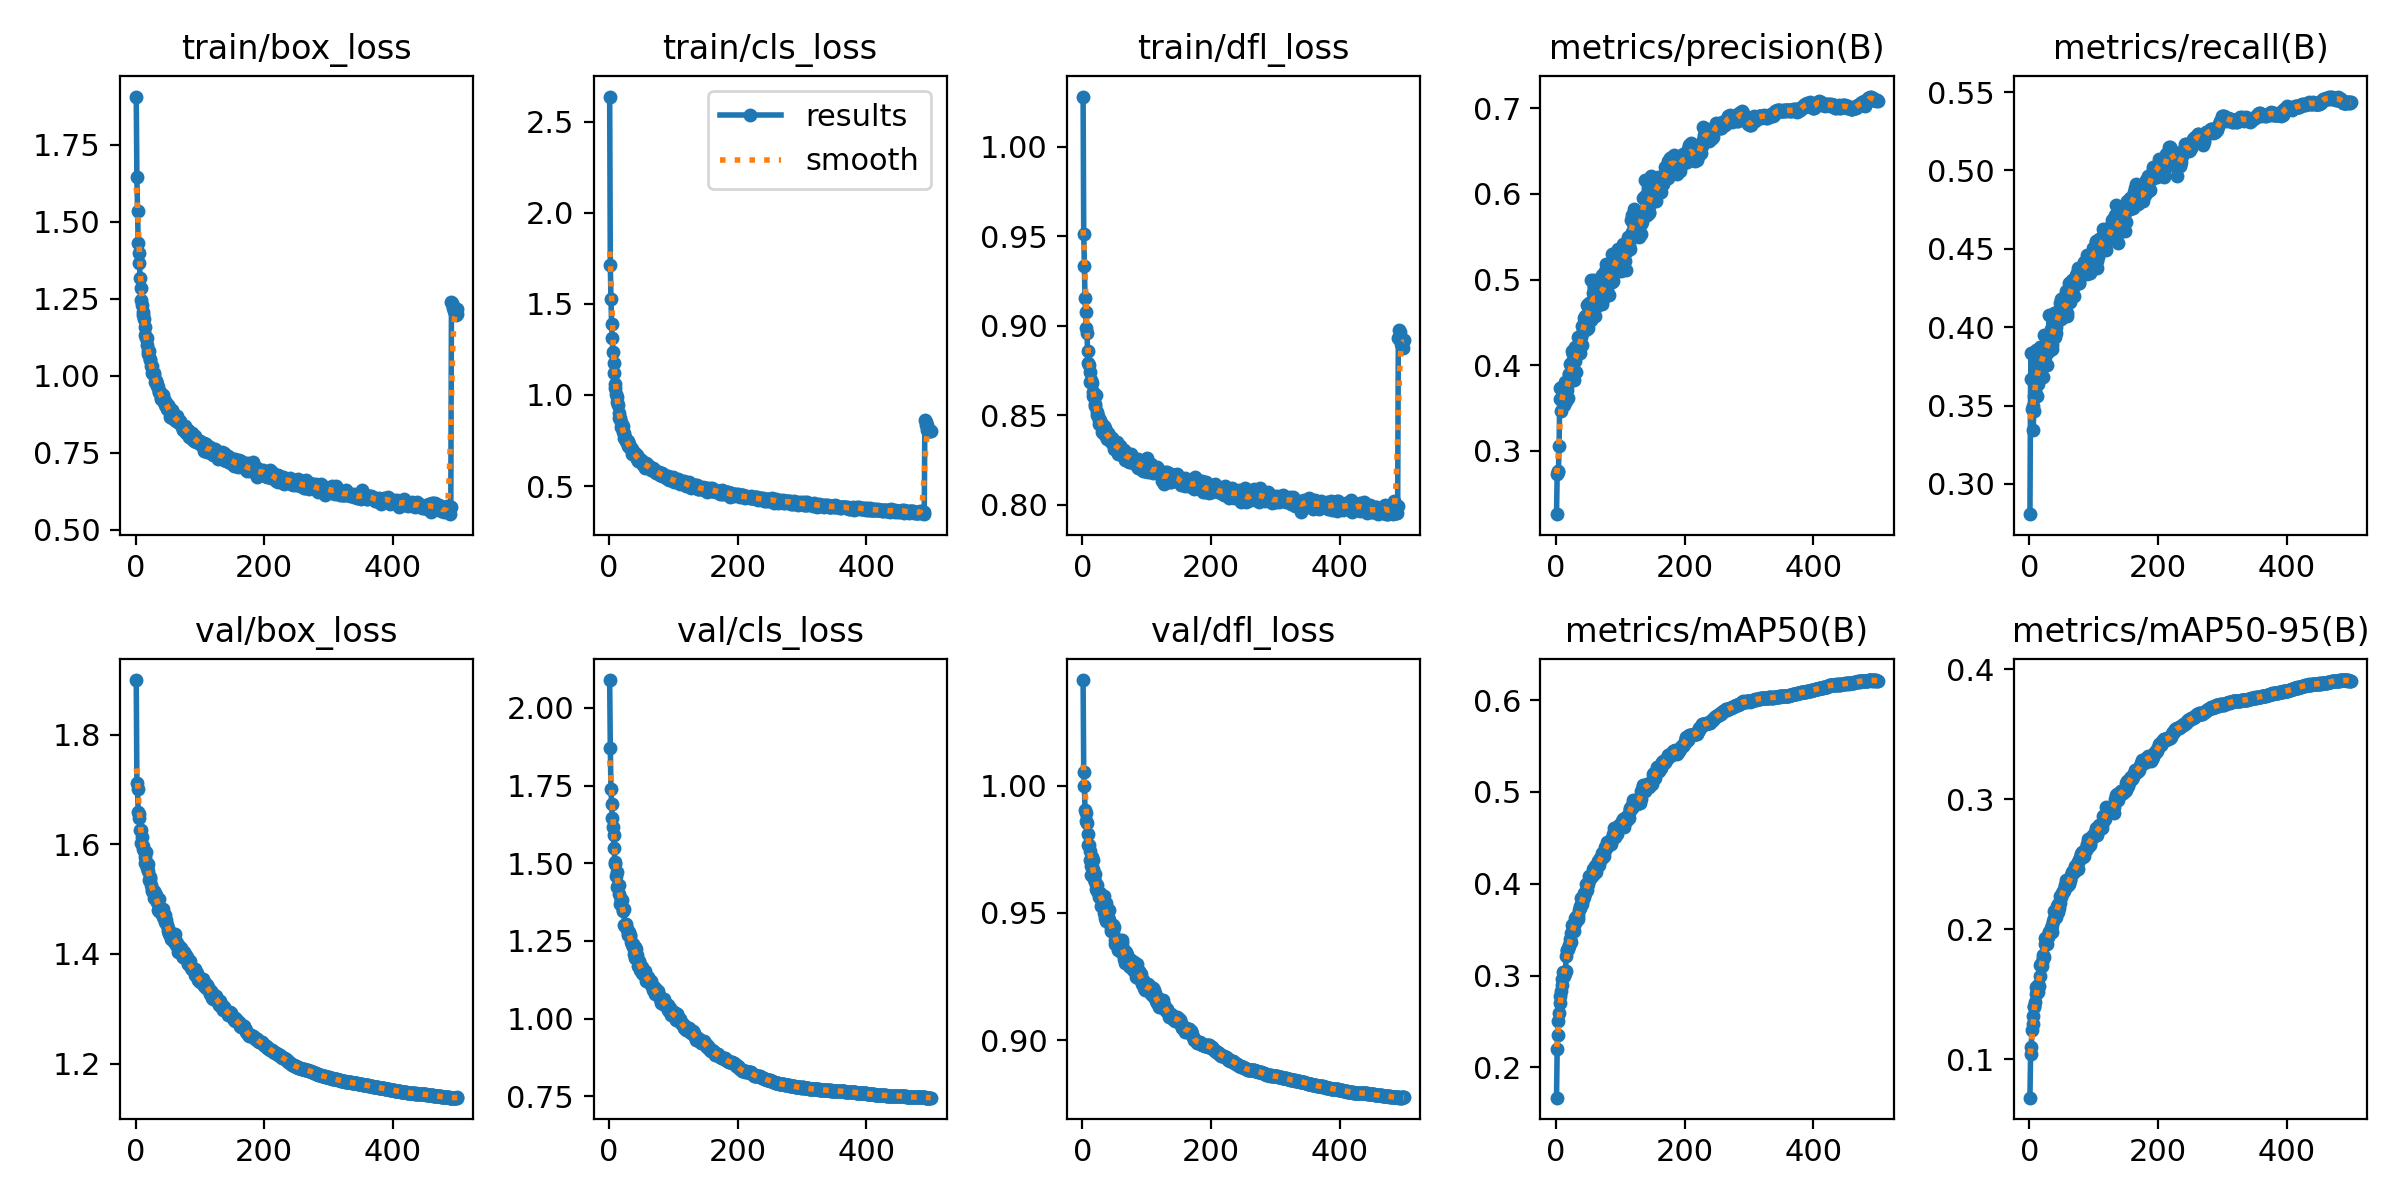
\includegraphics[width=0.8\textwidth]{v_3/results.png}
        \caption{Andamento funzioni di loss e metriche durante l'esecuzione di \texttt{medium-200-0}}
        \label{fig:v3-2}
    \end{figure}
    % - grafici recall e precision e performance e F1
    \begin{figure}[h]
        \centering
        \begin{subfigure}{.5\textwidth}
            \centering
            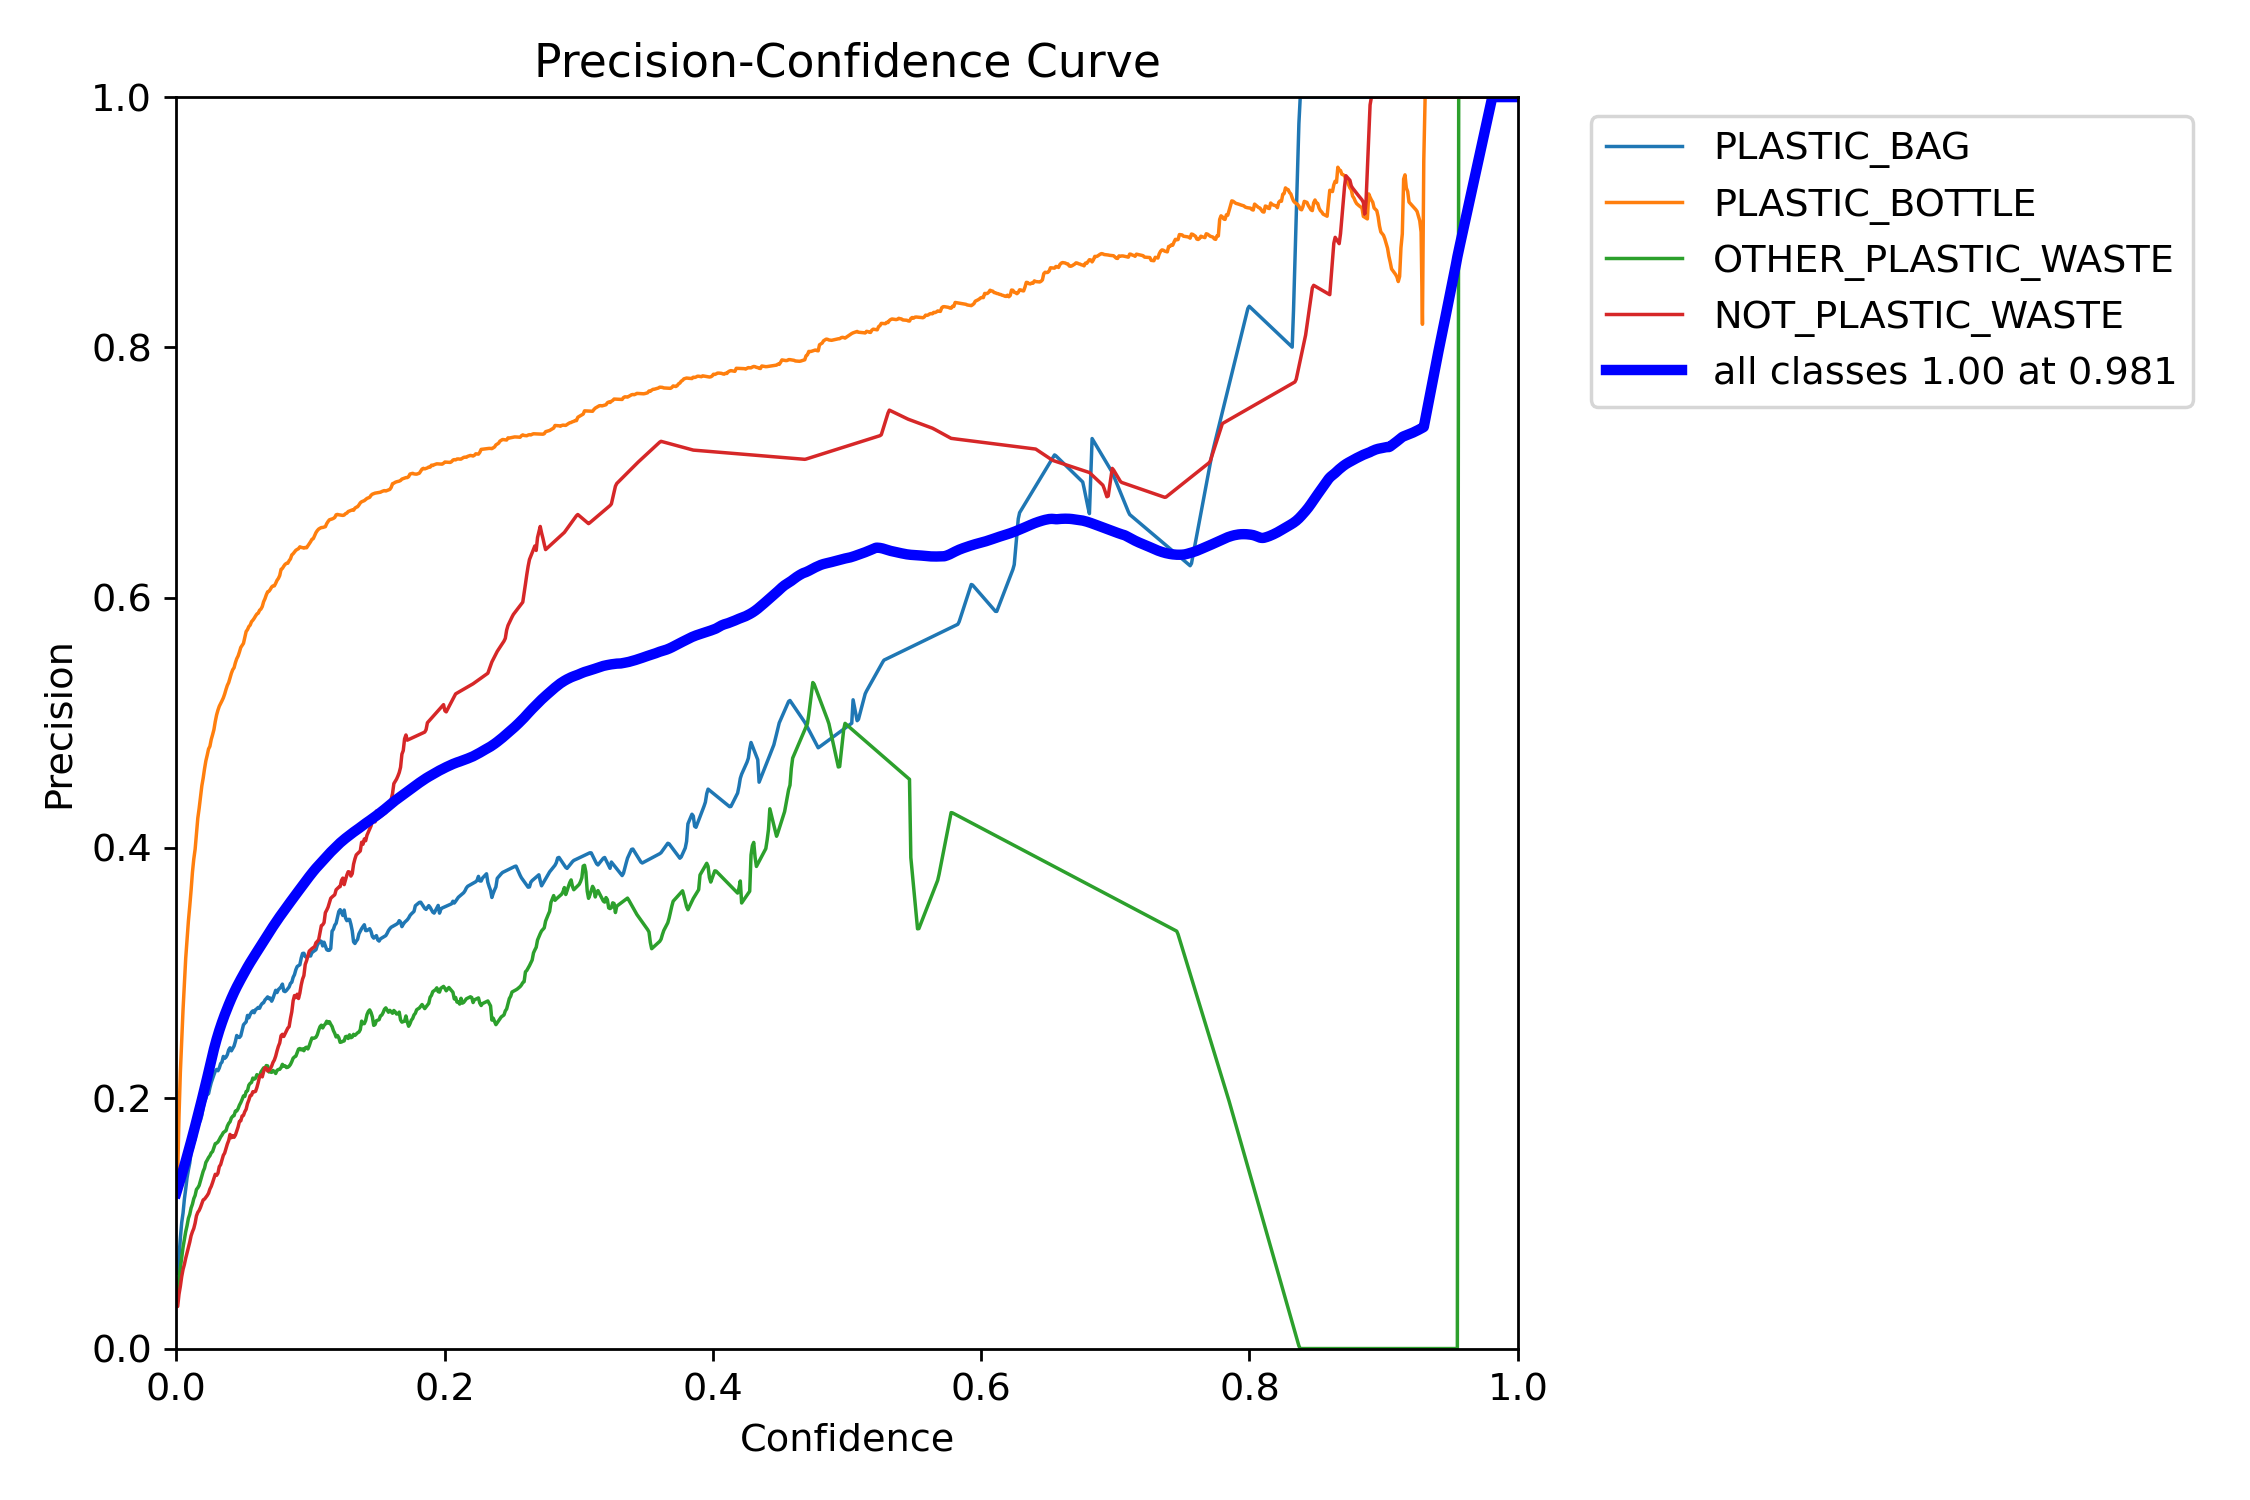
\includegraphics[width=.9\linewidth]{v_3/P_curve.png}
            
            \label{fig:v3-3.1}
          \end{subfigure}%
          \begin{subfigure}{.5\textwidth}
            \centering
            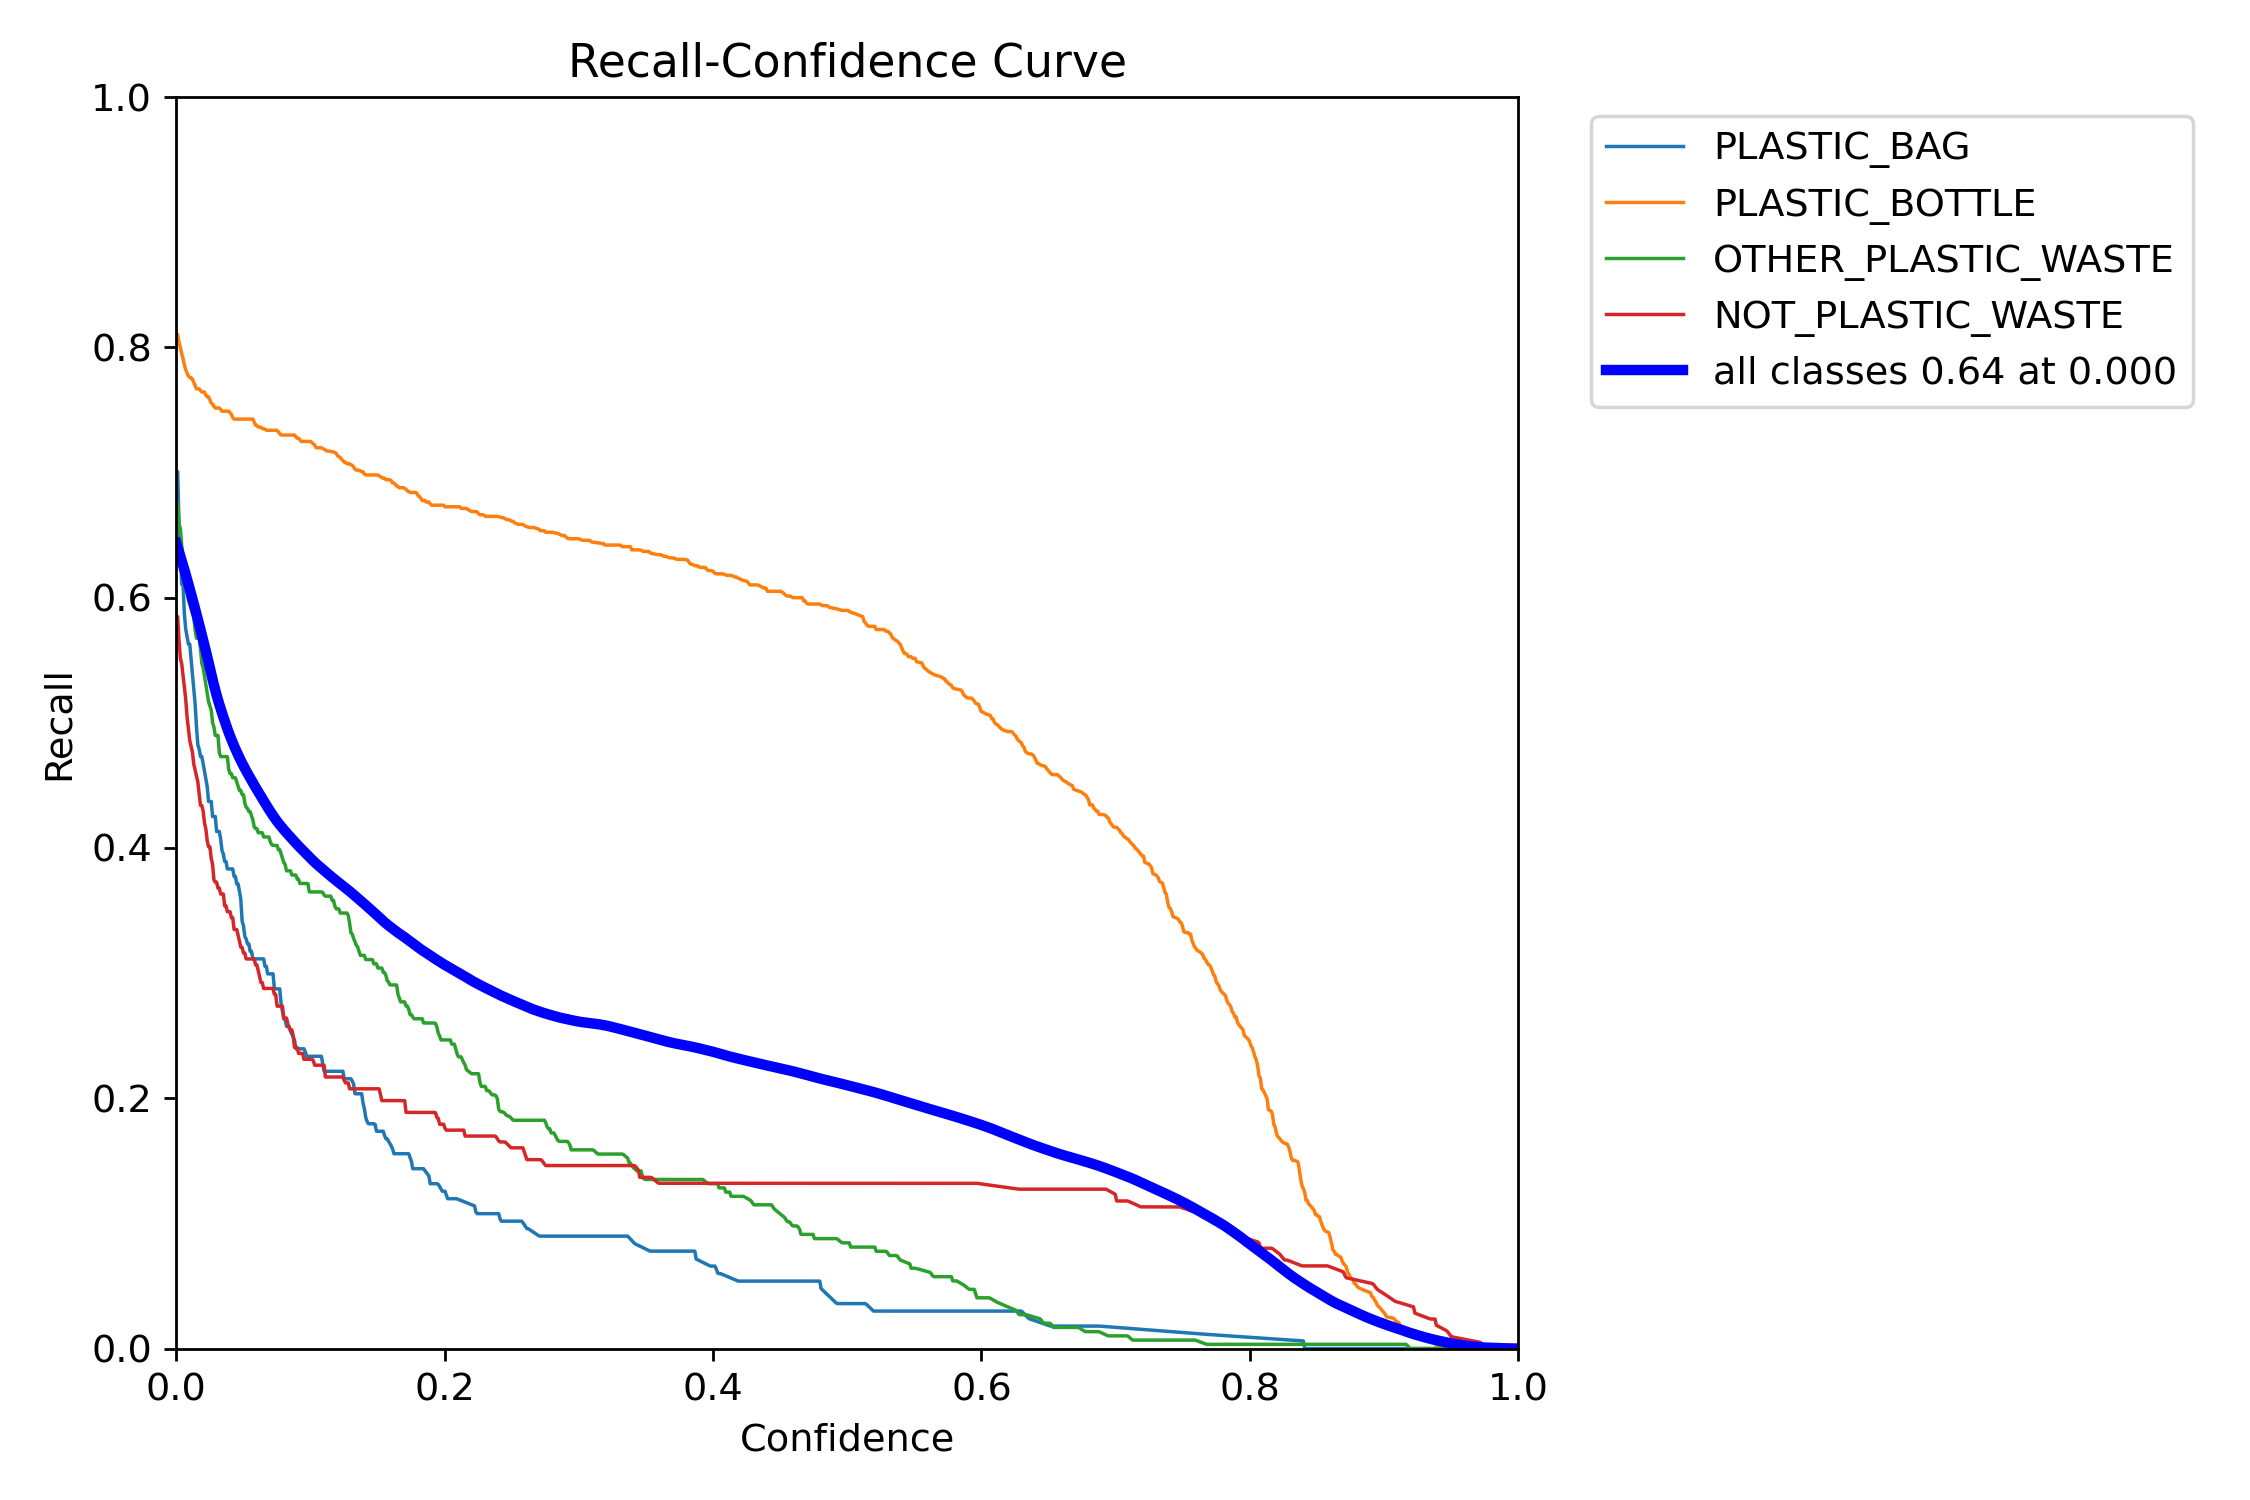
\includegraphics[width=.9\linewidth]{v_3/R_curve.png}
            
            \label{fig:v3-3.2}
          \end{subfigure}
          \vskip\baselineskip
        \begin{subfigure}{.5\textwidth}
          \centering
          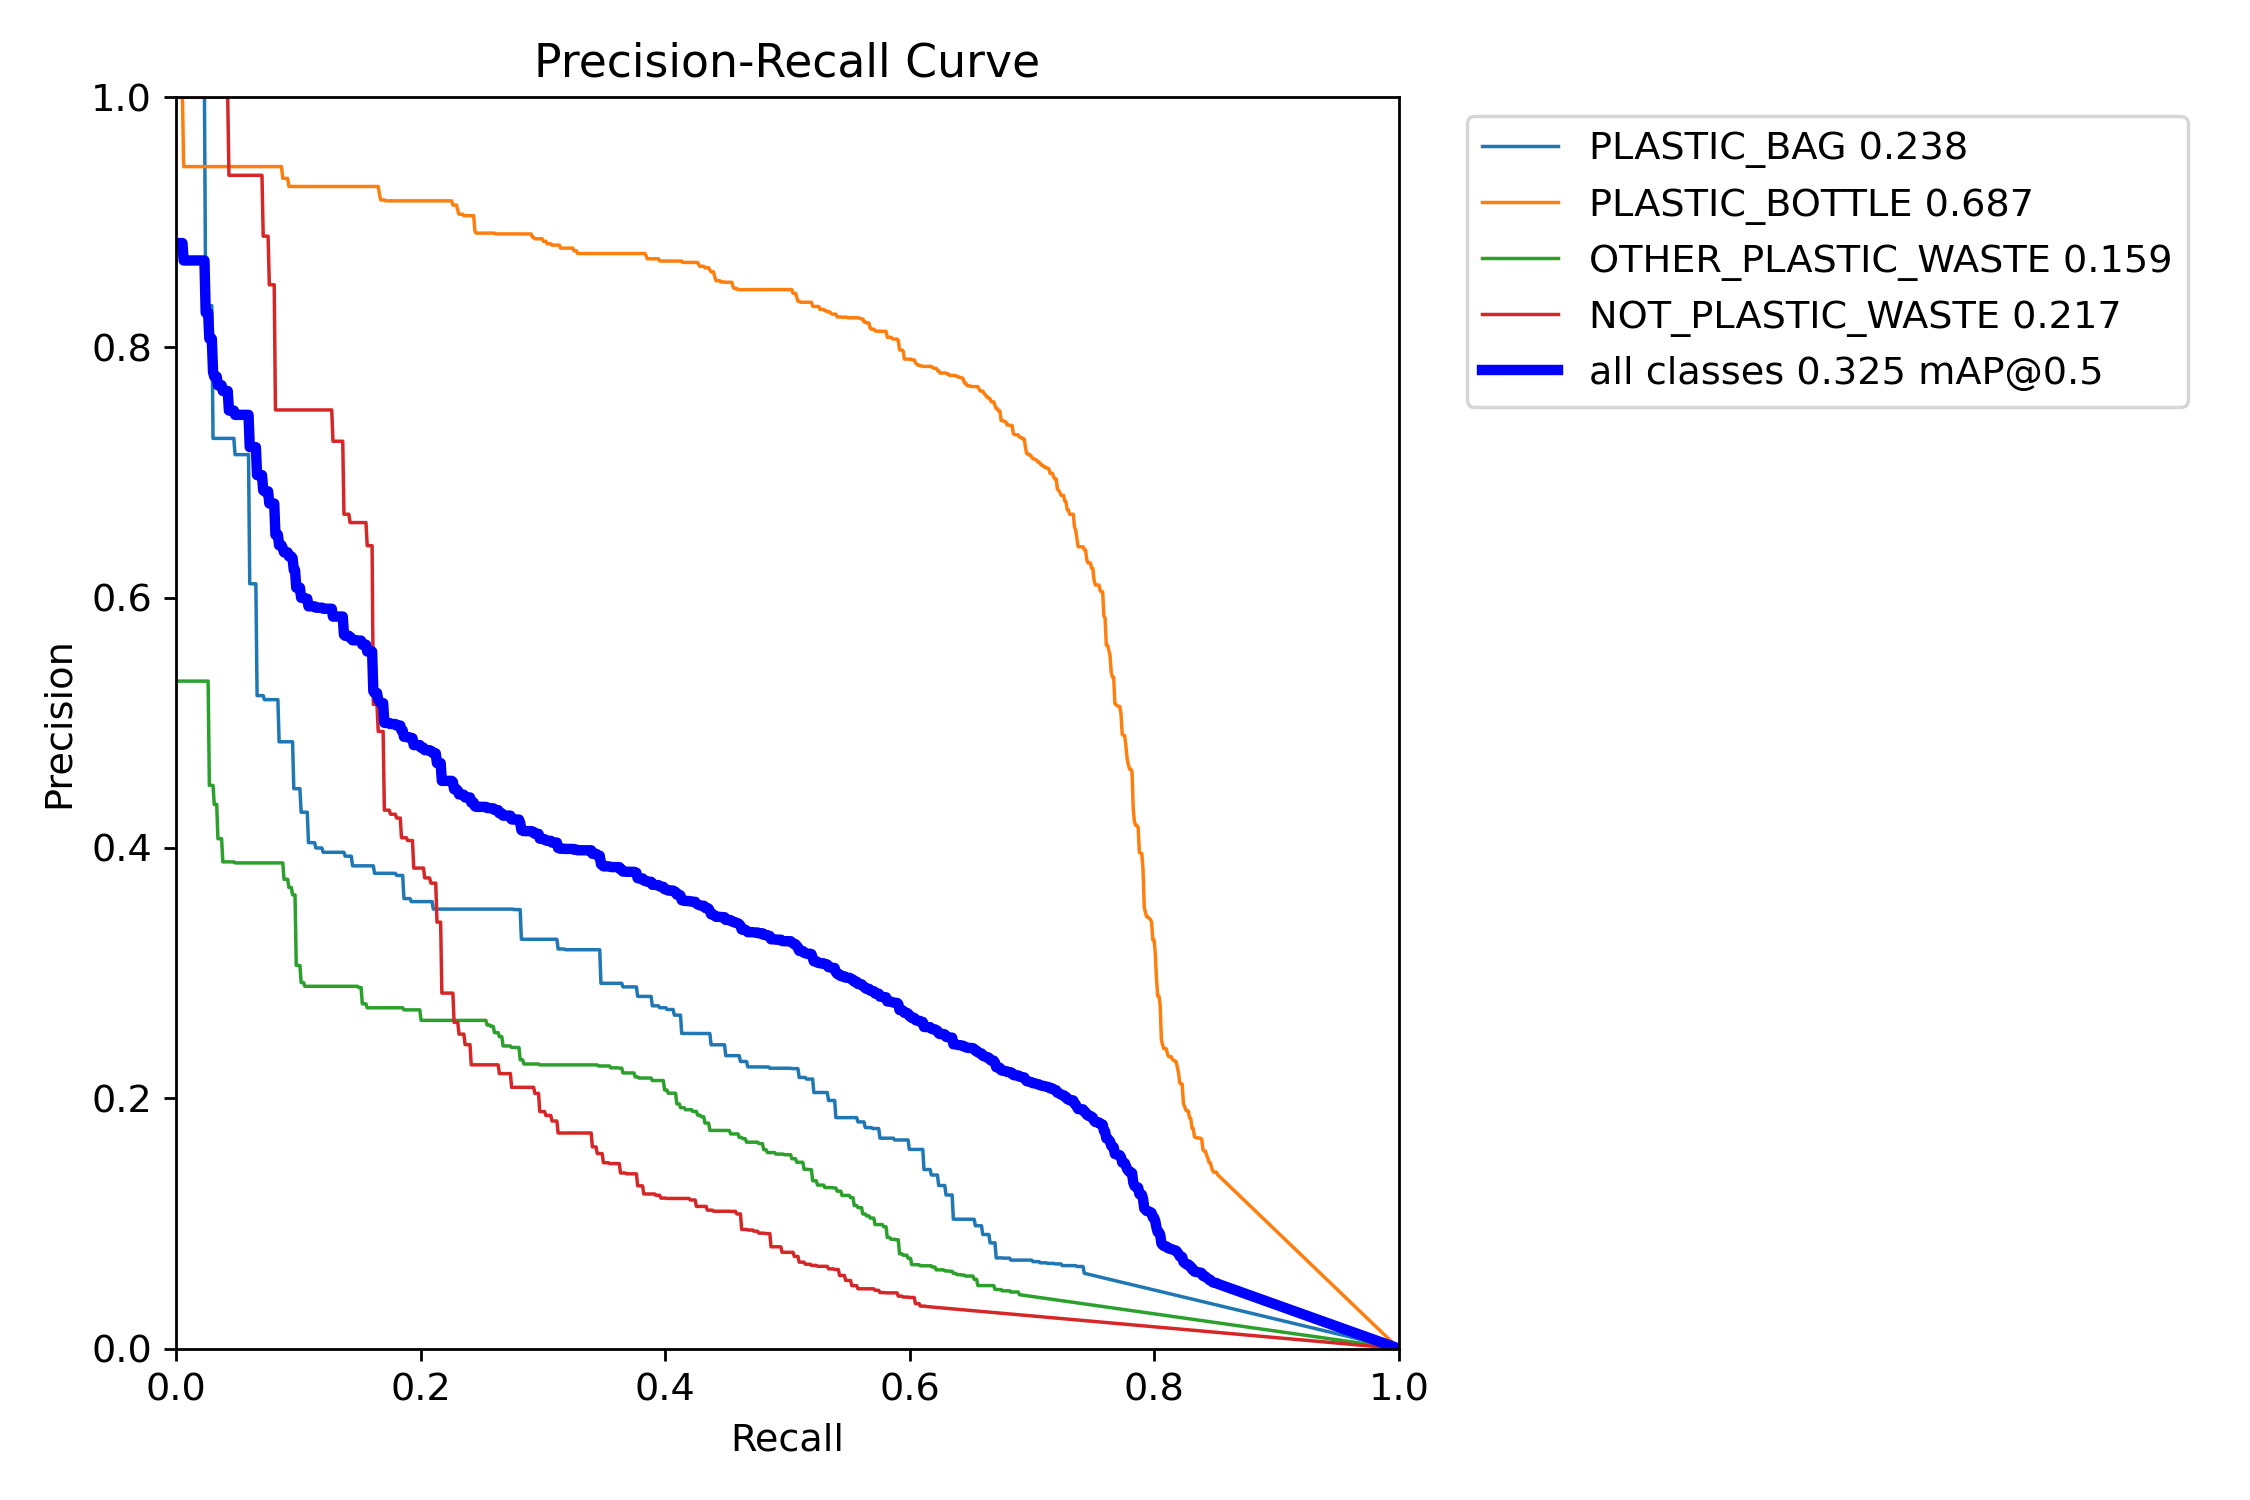
\includegraphics[width=.9\linewidth]{v_3/PR_curve.png}
          \label{fig:v3-3.3}
        \end{subfigure}
        \begin{subfigure}{.49\textwidth}
            \centering
            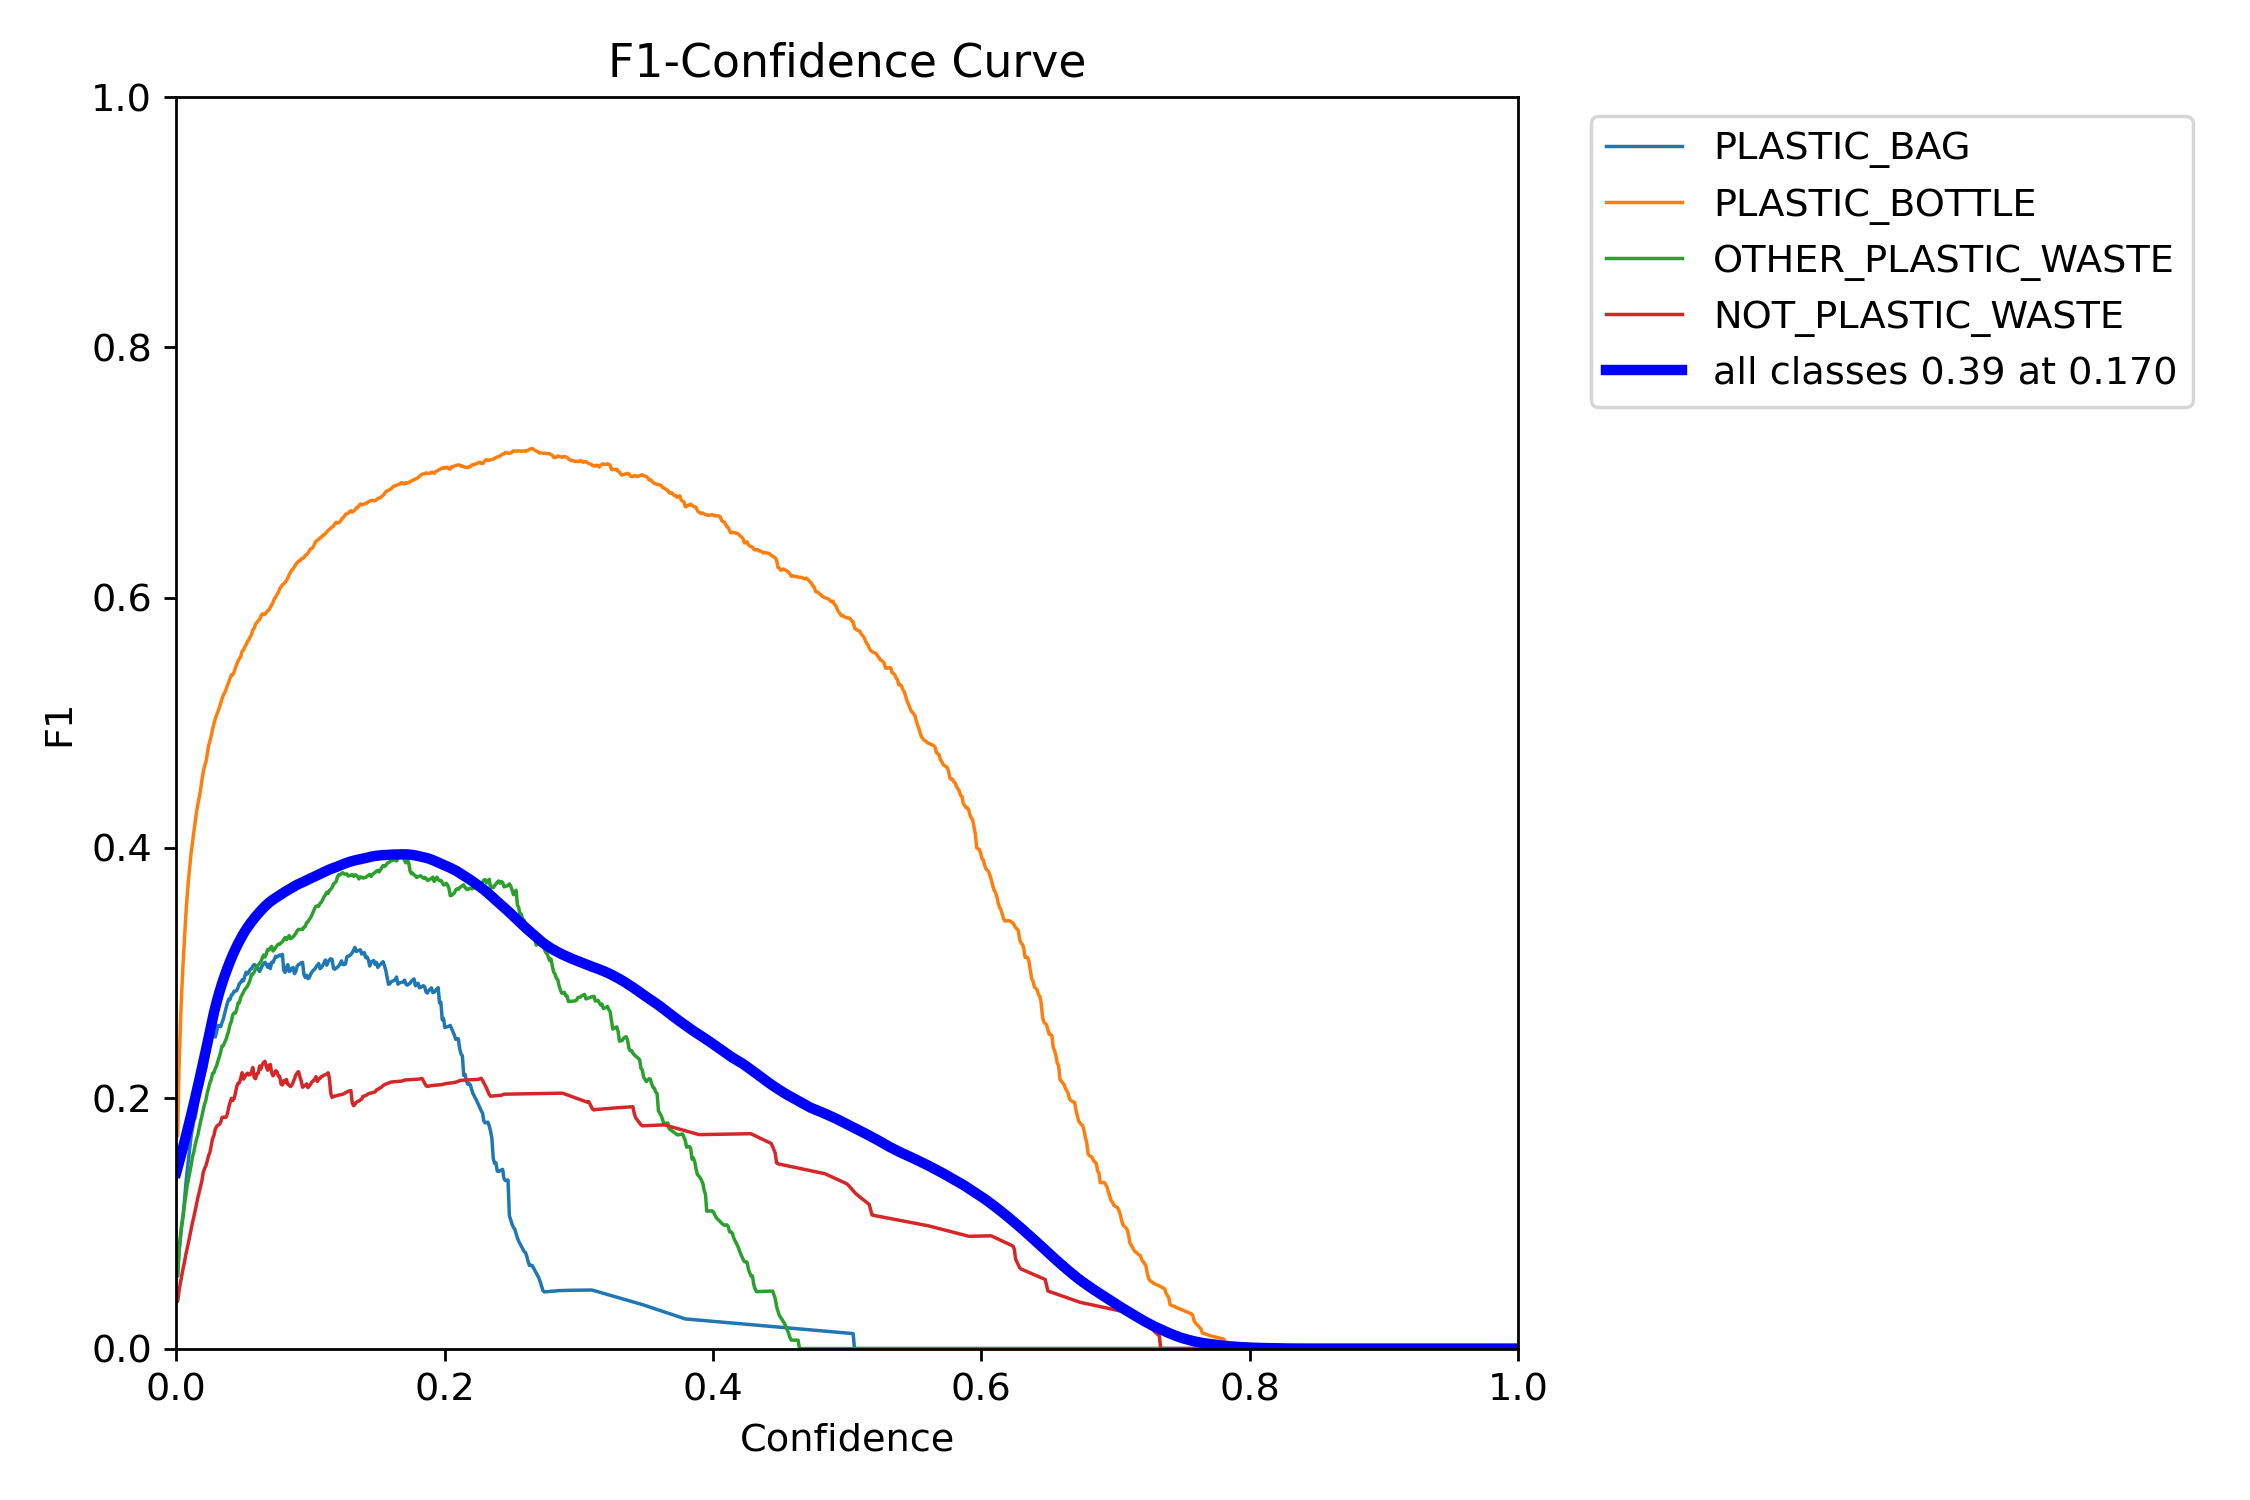
\includegraphics[width=.9\linewidth]{v_3/F1_curve.png}
            \label{fig:v3-3.4}
          \end{subfigure}

        \caption{Andamento funzioni di loss e metriche durante l'esecuzione di \texttt{medium-200-0}}
        \label{fig:v3-3}
    \end{figure}


    % - matrici di confusione
    \begin{figure}[h]
        \centering
        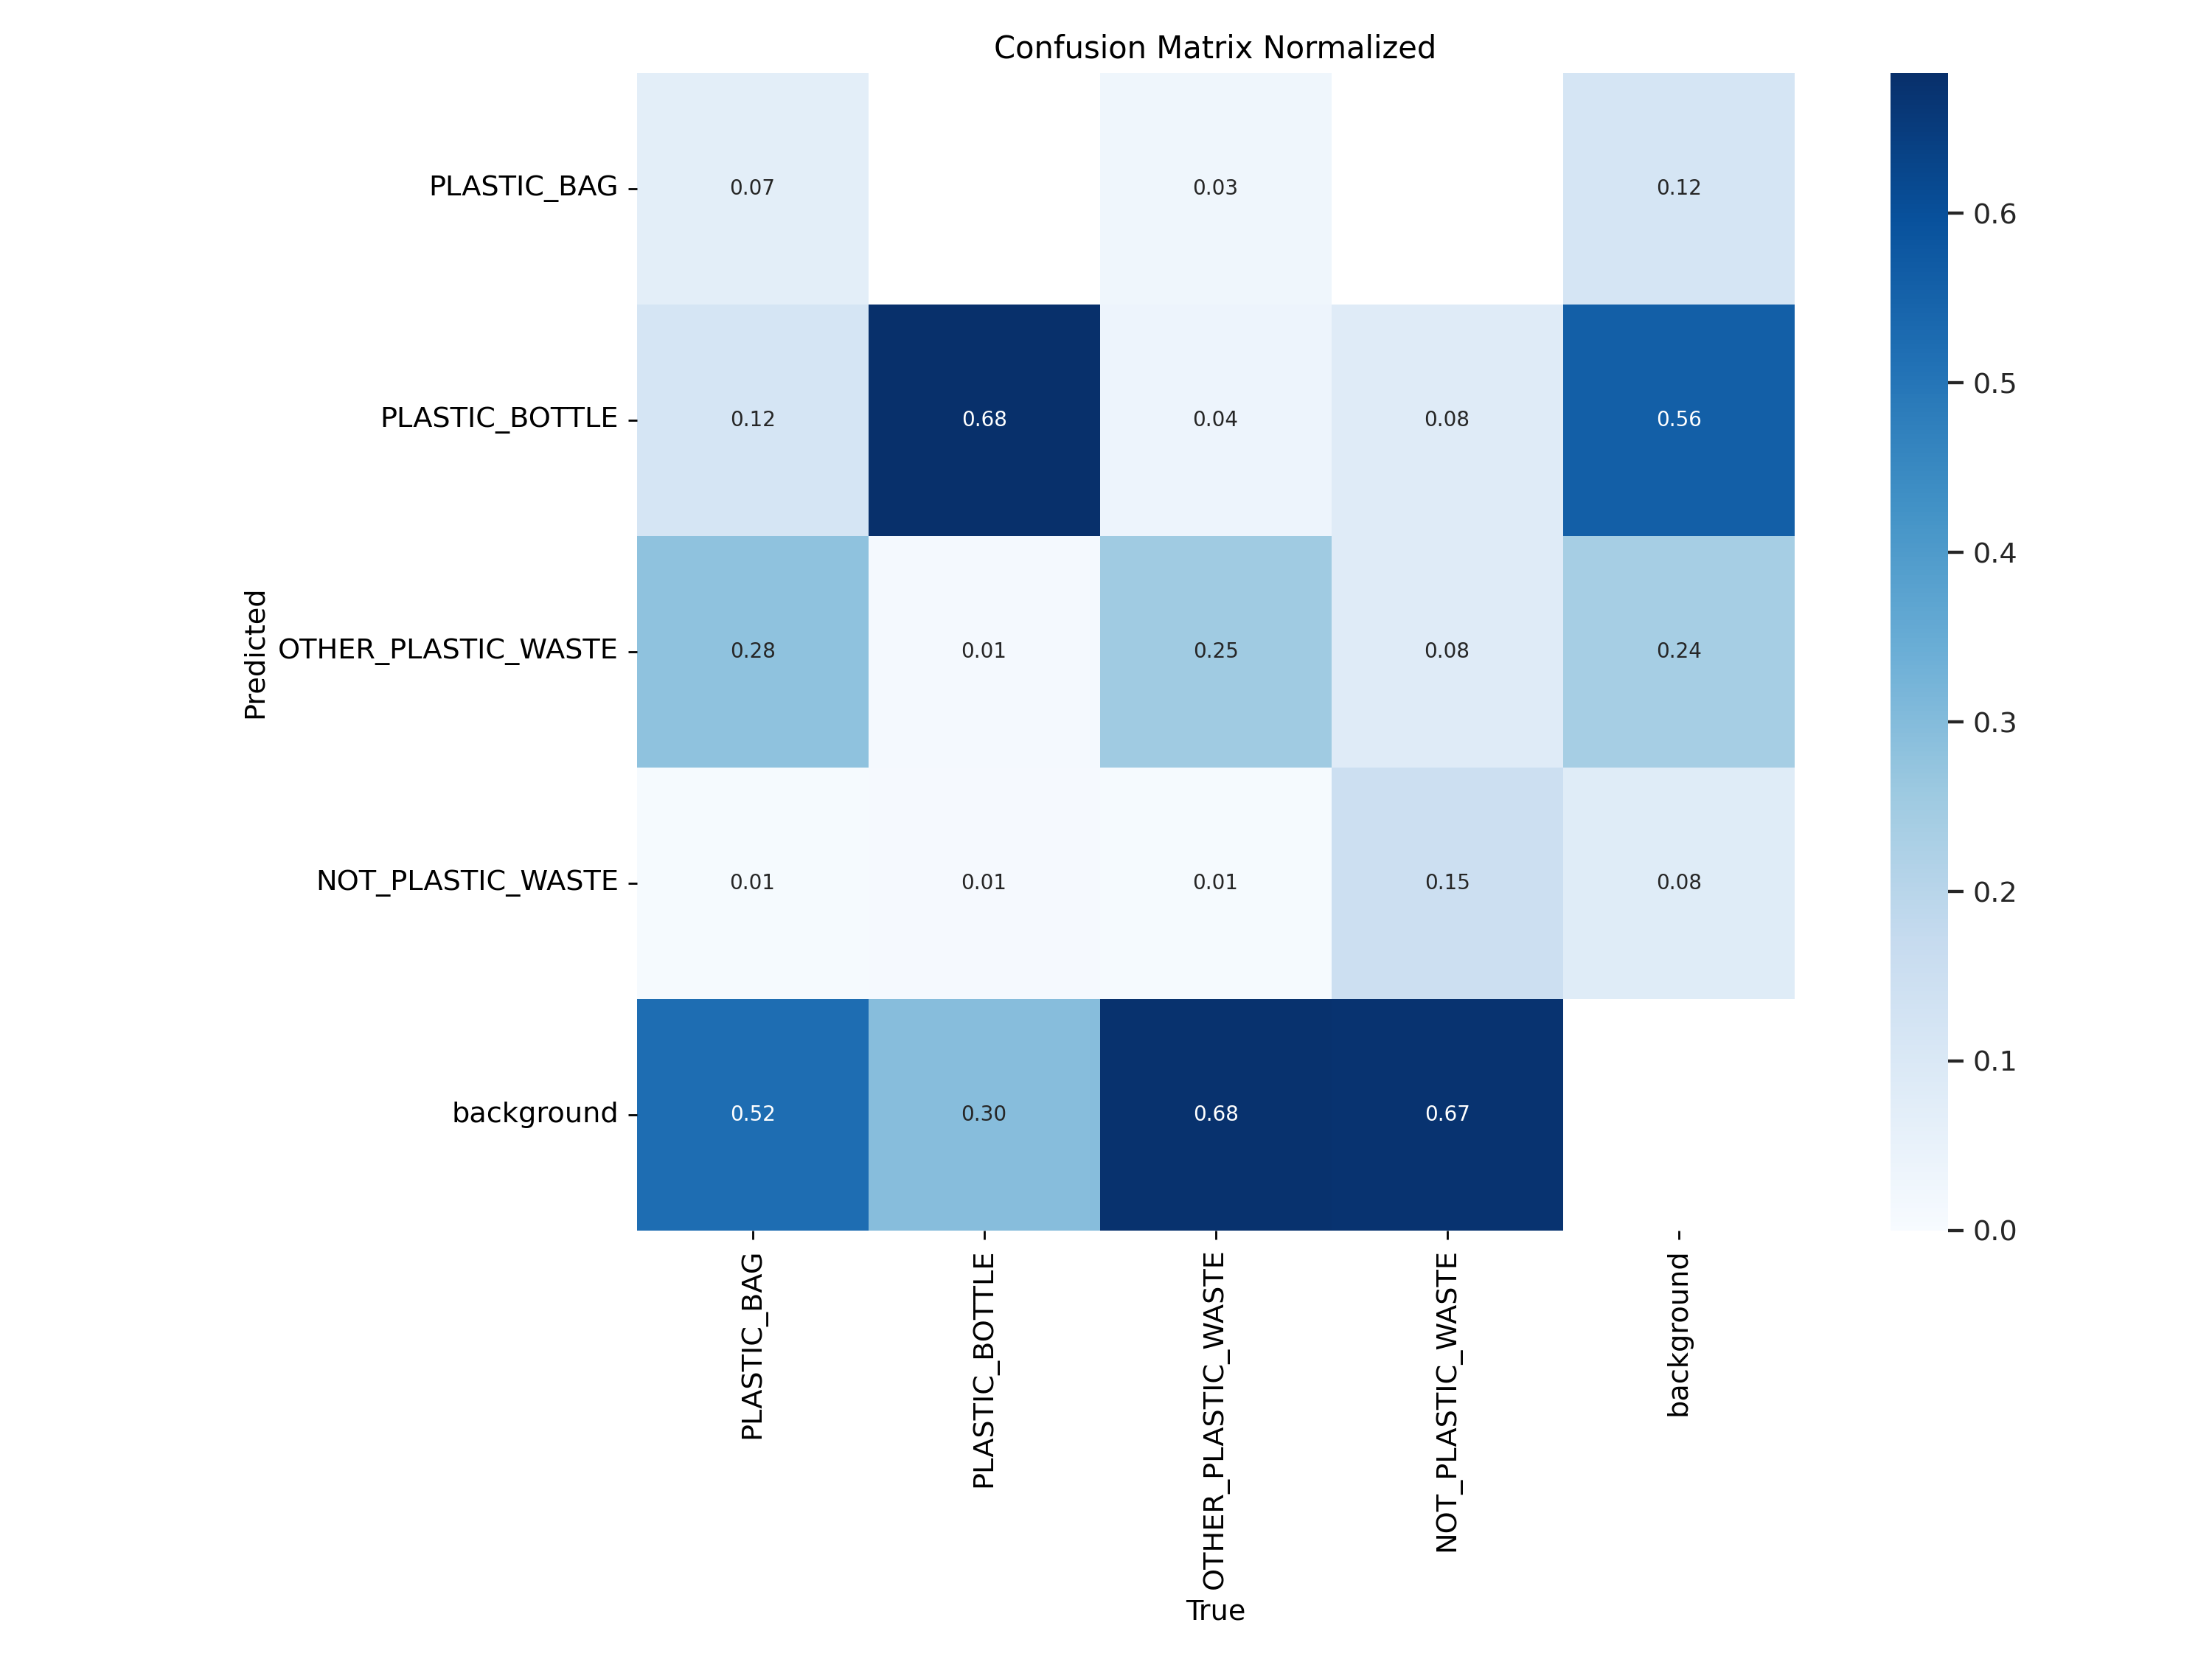
\includegraphics[width=0.8\textwidth]{v_3/confusion_matrix_normalized.png}
        \caption{Matrice di confusione normalizzata data dal modello \texttt{medium-200-0}}
        \label{fig:v3-4}
    \end{figure}
    % - tabella performance test set

